\chapter{Функциональные запросы}

Для проверки работы базы данных был подготовлен файл \texttt{queries.sql}. В нем находится десять SQL-запросов. Они показывают простые выборки, фильтрацию, объединение таблиц, группировку, агрегатные функции, условие \texttt{HAVING}, обобщенное табличное выражение \texttt{WITH}, сортировку и ограничение результата.

\section{Запрос 1}

Первый запрос выводит список всех абонентов. Он показывает идентификатор абонента, ФИО, email и статус. Такой запрос нужен для просмотра общего реестра клиентов оператора.

\begin{lstlisting}
SELECT subscriber_id, full_name, email, status
FROM subscribers;
\end{lstlisting}

\begin{figure}[H]
    \centering
    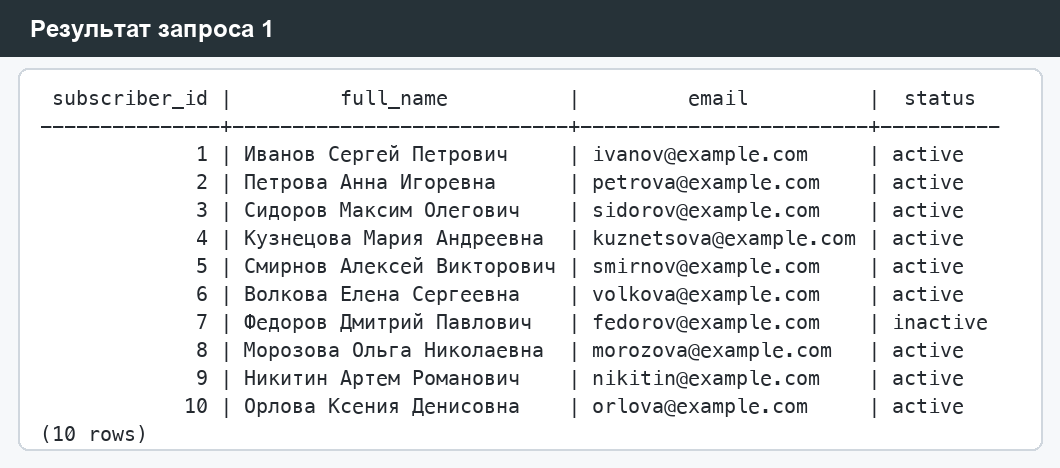
\includegraphics[width=\textwidth]{screen1.png}
    \caption{Результат запроса 1: список абонентов}
\end{figure}

\section{Запрос 2}

Второй запрос выводит список тарифных планов. В результате видны название тарифа, ежемесячная плата, объем интернета, количество минут и SMS.

\begin{lstlisting}
SELECT tariff_id, tariff_name, monthly_fee, internet_gb, minutes_count, sms_count
FROM tariffs;
\end{lstlisting}

\begin{figure}[H]
    \centering
    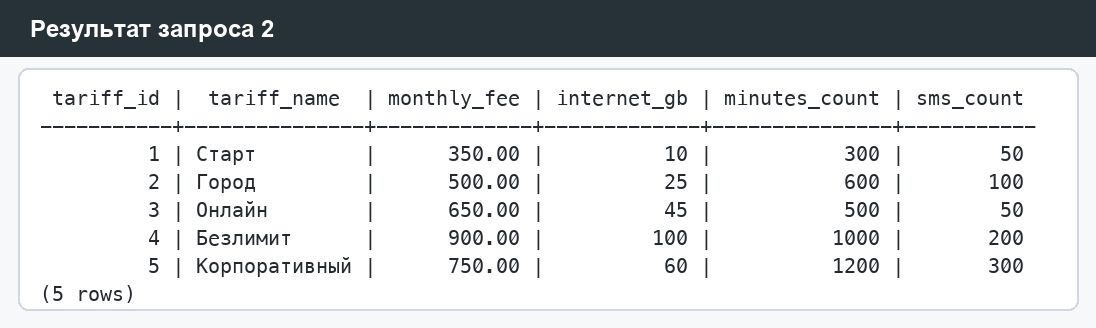
\includegraphics[width=\textwidth]{screen2.png}
    \caption{Результат запроса 2: список тарифов}
\end{figure}

\section{Запрос 3}

Третий запрос ищет свободные телефонные номера. Для этого используется условие \texttt{WHERE status = 'available'}. Такой запрос может использовать сотрудник перед выдачей нового номера абоненту.

\begin{lstlisting}
SELECT phone_number_id, msisdn, region_name
FROM phone_numbers
WHERE status = 'available';
\end{lstlisting}

\begin{figure}[H]
    \centering
    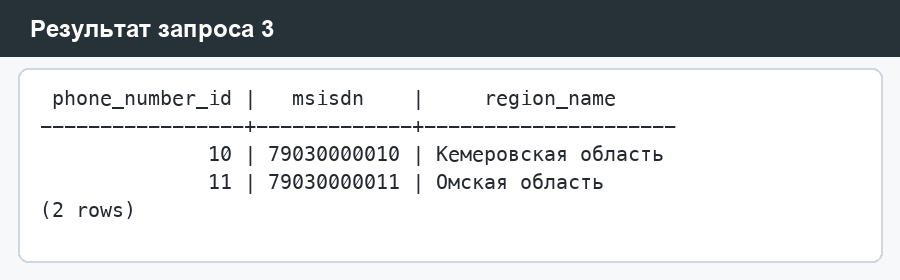
\includegraphics[width=\textwidth]{screen3.png}
    \caption{Результат запроса 3: свободные телефонные номера}
\end{figure}

\section{Запрос 4}

Четвертый запрос выводит заблокированные SIM-карты. Он помогает быстро найти SIM-карты, которые нельзя использовать для новой выдачи.

\begin{lstlisting}
SELECT sim_card_id, iccid, imsi, status
FROM sim_cards
WHERE status = 'blocked';
\end{lstlisting}

\begin{figure}[H]
    \centering
    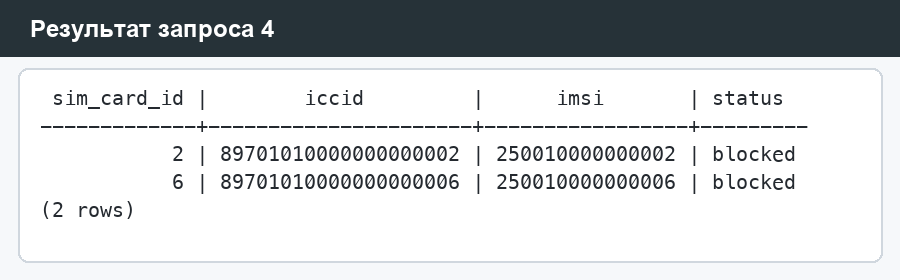
\includegraphics[width=\textwidth]{screen4.png}
    \caption{Результат запроса 4: заблокированные SIM-карты}
\end{figure}

\section{Запрос 5}

Пятый запрос выбирает операции за март 2026 года. Здесь используется фильтрация по диапазону дат. Такой запрос нужен для просмотра действий за конкретный период.

\begin{lstlisting}
SELECT operation_id, operation_type, operation_time, details
FROM operation_history
WHERE operation_time >= '2026-03-01' AND operation_time < '2026-04-01';
\end{lstlisting}

\begin{figure}[H]
    \centering
    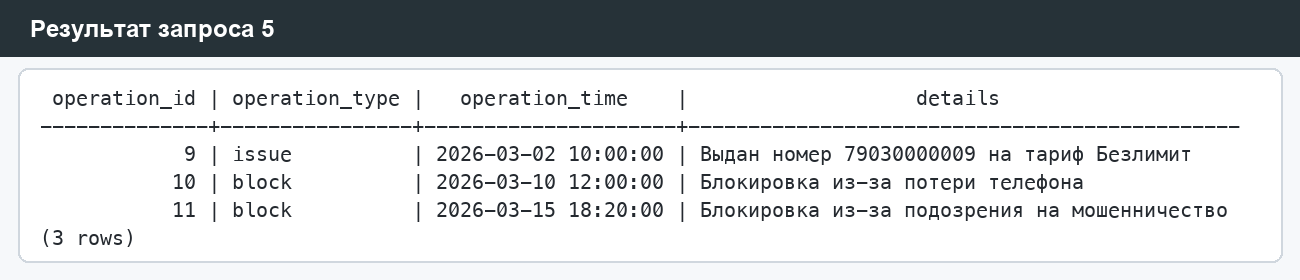
\includegraphics[width=\textwidth]{screen5.png}
    \caption{Результат запроса 5: операции за март 2026 года}
\end{figure}

\section{Запрос 6}

Шестой запрос формирует сводный список активных выдач. В нем используется несколько соединений \texttt{JOIN}, чтобы показать ФИО абонента, номер телефона, ICCID SIM-карты, тариф и дату начала обслуживания.

\begin{lstlisting}
SELECT s.full_name, pn.msisdn, sc.iccid, t.tariff_name, na.start_date
FROM number_assignments na
JOIN subscribers s ON s.subscriber_id = na.subscriber_id
JOIN phone_numbers pn ON pn.phone_number_id = na.phone_number_id
JOIN sim_cards sc ON sc.sim_card_id = na.sim_card_id
JOIN tariffs t ON t.tariff_id = na.tariff_id
WHERE na.status = 'active'
ORDER BY s.full_name;
\end{lstlisting}

\begin{figure}[H]
    \centering
    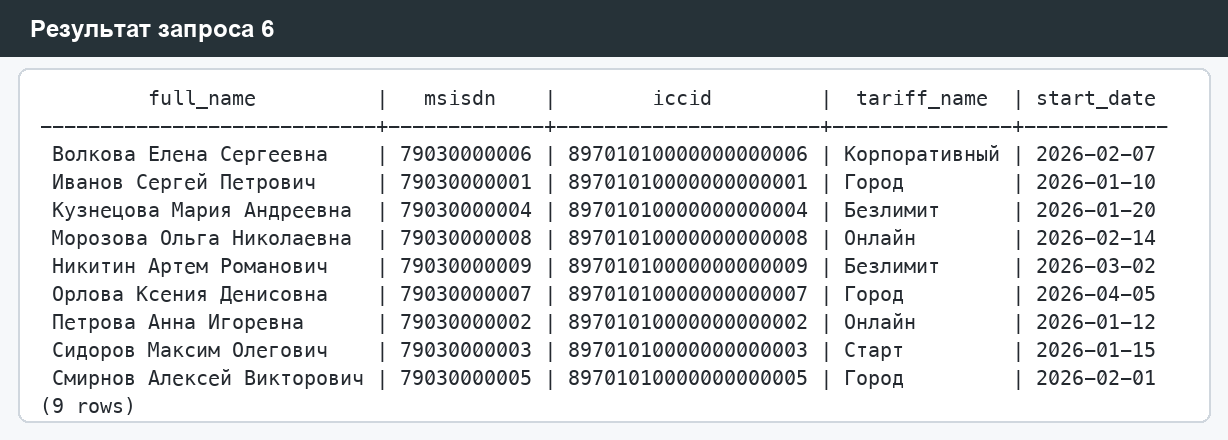
\includegraphics[width=\textwidth]{screen6.png}
    \caption{Результат запроса 6: активные выдачи номеров}
\end{figure}

\section{Запрос 7}

Седьмой запрос выводит отчет по блокировкам. Он соединяет таблицы блокировок, выдач, абонентов и номеров. В результате видно, какой абонент был заблокирован, по какому номеру, по какой причине и когда была выполнена разблокировка.

\begin{lstlisting}
SELECT br.block_id, s.full_name, pn.msisdn, br.reason_text, br.blocked_at, br.unblocked_at, br.status
FROM block_requests br
JOIN number_assignments na ON na.assignment_id = br.assignment_id
JOIN subscribers s ON s.subscriber_id = na.subscriber_id
JOIN phone_numbers pn ON pn.phone_number_id = na.phone_number_id
ORDER BY br.blocked_at DESC;
\end{lstlisting}

\begin{figure}[H]
    \centering
    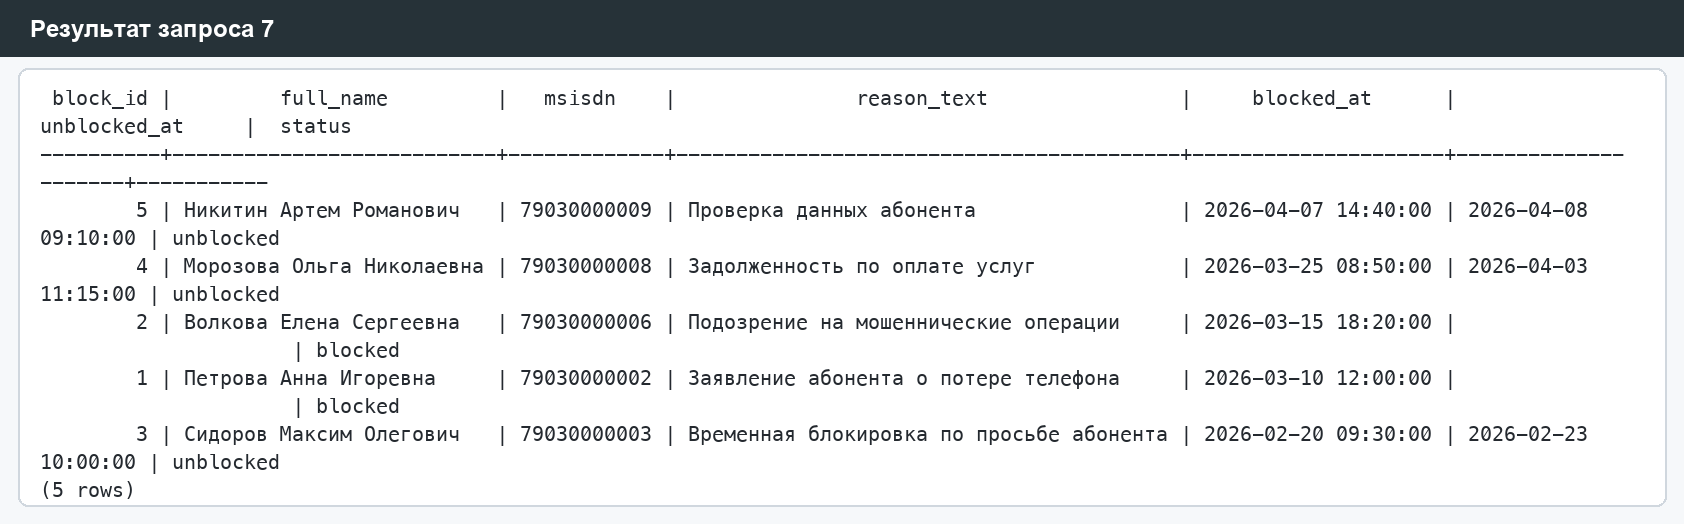
\includegraphics[width=\textwidth]{screen7.png}
    \caption{Результат запроса 7: отчет по блокировкам}
\end{figure}

\section{Запрос 8}

Восьмой запрос группирует телефонные номера по статусам и считает количество номеров в каждой группе. Здесь используется \texttt{GROUP BY} и функция \texttt{COUNT}.

\begin{lstlisting}
SELECT status, COUNT(*) AS numbers_count
FROM phone_numbers
GROUP BY status
ORDER BY numbers_count DESC;
\end{lstlisting}

\begin{figure}[H]
    \centering
    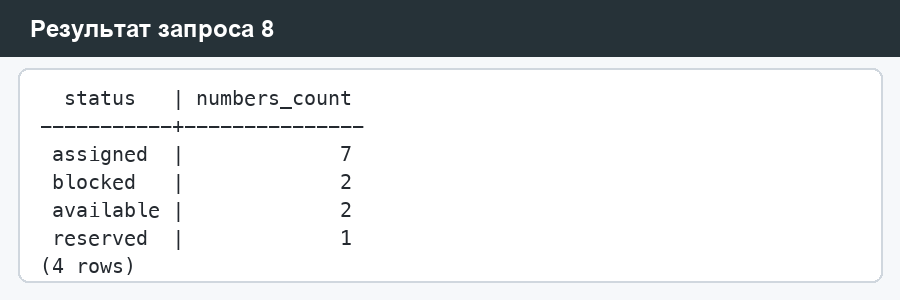
\includegraphics[width=\textwidth]{screen8.png}
    \caption{Результат запроса 8: количество номеров по статусам}
\end{figure}

\section{Запрос 9}

Девятый запрос считает количество активных выдач по тарифам и ожидаемую ежемесячную выручку. В запросе используется \texttt{GROUP BY}, \texttt{SUM} и условие \texttt{HAVING}, которое оставляет только тарифы с количеством активных выдач больше одного.

\begin{lstlisting}
SELECT t.tariff_name, COUNT(*) AS active_assignments, SUM(t.monthly_fee) AS expected_monthly_income
FROM number_assignments na
JOIN tariffs t ON t.tariff_id = na.tariff_id
WHERE na.status = 'active'
GROUP BY t.tariff_name
HAVING COUNT(*) > 1
ORDER BY expected_monthly_income DESC;
\end{lstlisting}

\begin{figure}[H]
    \centering
    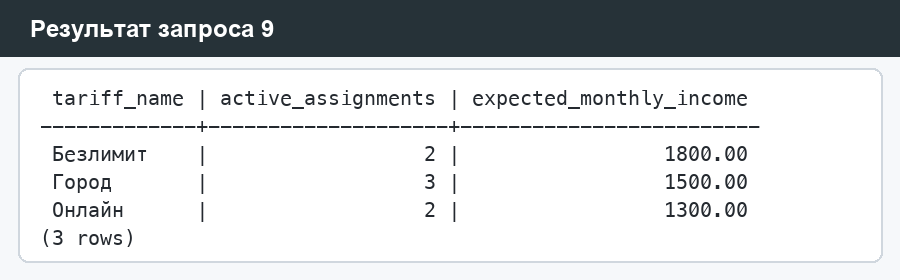
\includegraphics[width=\textwidth]{screen9.png}
    \caption{Результат запроса 9: аналитика по активным тарифам}
\end{figure}

\section{Запрос 10}

Десятый запрос показывает топ-5 абонентов по количеству операций. В нем используется обобщенное табличное выражение \texttt{WITH}, сортировка \texttt{ORDER BY} и ограничение \texttt{LIMIT}. Такой запрос полезен для анализа наиболее активных абонентов.

\begin{lstlisting}
WITH subscriber_operations AS (
    SELECT s.subscriber_id, s.full_name, COUNT(oh.operation_id) AS operations_count
    FROM subscribers s
    JOIN number_assignments na ON na.subscriber_id = s.subscriber_id
    JOIN operation_history oh ON oh.assignment_id = na.assignment_id
    GROUP BY s.subscriber_id, s.full_name
)
SELECT full_name, operations_count
FROM subscriber_operations
ORDER BY operations_count DESC, full_name
LIMIT 5;
\end{lstlisting}

\begin{figure}[H]
    \centering
    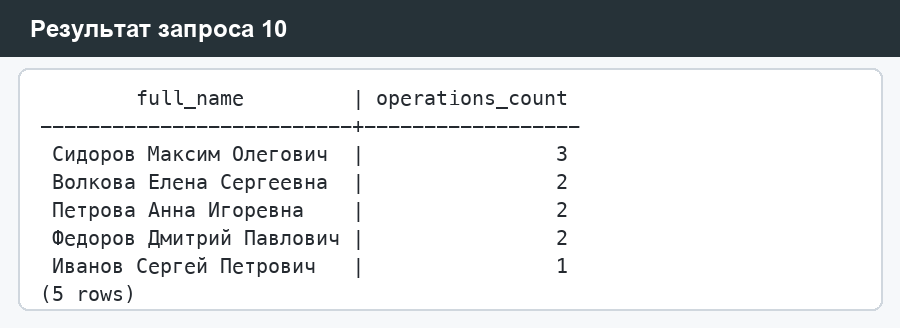
\includegraphics[width=\textwidth]{screen10.png}
    \caption{Результат запроса 10: топ абонентов по количеству операций}
\end{figure}

\chapter*{Заключение}
\addcontentsline{toc}{chapter}{Заключение}

В результате расчетно-графической работы была разработана база данных для управления SIM-картами и телефонными номерами. В базе реализованы основные сущности предметной области, связи между ними, ограничения целостности и индексы. Также была подготовлена ER-диаграмма, тестовые данные и набор функциональных запросов.

Проект был дополнительно упакован в Docker Compose. Благодаря этому PostgreSQL можно запустить одной командой, а структура и тестовые данные создаются автоматически. Все запросы были проверены в контейнере и вернули корректные результаты. Поэтому разработанная база данных соответствует требованиям расчетно-графической работы.
